\chapter[Helicidade zero]{Extensão escalar vinculada de Fierz--Pauli: inferência condicional}
\label{cap:c10-parcial}

\noindent\textbf{Estado: campanha condicional concluída; limitações numéricas explicitadas.}

Este capítulo reúne a extensão teórica e os componentes numéricos já desenvolvidos para incluir a helicidade zero de Fierz--Pauli. Há uma derivação da resposta observável, verificações independentes da função de redução de sobreposição (ORF) e um resultado negativo de interpolação que restringe o uso desses cálculos. O primeiro piloto físico escalar foi executado em 16 dados fixos de engenharia. Suas verificações de integração identificaram falhas que motivaram refinamentos preservando os caches. A campanha populacional subsequente concluiu 6.344 análises, com falsos positivos, recuperação, calibração e degenerescências locais avaliados no domínio condicional declarado. Os casos numericamente indeterminados permanecem nos resultados.

\section{Uma amplitude escalar e seus vínculos}

Mantêm-se a assinatura $(+---)$, a perturbação covariante $g_{\mu\nu}=\eta_{\mu\nu}+H_{\mu\nu}$ e a fase $\exp[i\omega(t-\beta\widehat\Omega\cdot\boldsymbol{x}/c)]$. A direção $\widehat\Omega$ aponta no sentido de propagação, enquanto $\boldsymbol p_a$ aponta da Terra para o pulsar. Definem-se
\begin{equation}
 \beta=\frac{ck}{\omega},\qquad
 \chi=1-\beta^2=\left(\frac{f_g}{f}\right)^2,
 \qquad y_a=\frac{\omega L_a}{c}.
\end{equation}
Para o modo massivo viajante, $0\leq\beta<1$. O ponto $\beta=0$ é o limiar; $\beta\to1$ será empregado apenas como limite formal da resposta.

Sejam $e^1_\mu,e^2_\mu$ dois vetores espaciais transversais ortonormais e
\begin{equation}
 U_\mu=\frac{(\beta,-\widehat\Omega)}{\sqrt\chi},
 \qquad U_\mu U^\mu=-1.
\end{equation}
Uma polarização real de helicidade zero, na mesma norma de Lorentz dois das polarizações reais tensoriais, é
\begin{equation}
 E^{(0)}_{\mu\nu}=\frac{e^1_\mu e^1_\nu+e^2_\mu e^2_\nu-2U_\mu U_\nu}{\sqrt3},
 \qquad H_{\mu\nu}=h_0E^{(0)}_{\mu\nu}.
\end{equation}
Ela satisfaz transversalidade em relação ao quadrimomento da onda, traço nulo e $E^{(0)}_{\mu\nu}E^{(0)\mu\nu}=2$. Escrevendo $P_{ij}=\delta_{ij}-\Omega_i\Omega_j$, suas componentes são
\begin{align}
 E^{(0)}_{00}&=-\frac{2\beta^2}{\sqrt3\chi},&
 E^{(0)}_{0i}&=\frac{2\beta\Omega_i}{\sqrt3\chi},\\
 E^{(0)}_{ij}&=\frac1{\sqrt3}\left(P_{ij}-\frac{2\Omega_i\Omega_j}{\chi}\right).
\end{align}
Existe uma amplitude física $h_0$. As deformações transversal escalar e longitudinal são componentes vinculadas dessa amplitude; atribuir-lhes potências independentes definiria outro modelo.

\section{Resposta de frequência com os observadores}

A presença de $H_{0\mu}$ exige incluir o movimento e a normalização dos observadores nos extremos do percurso. Esse requisito é consistente com a formulação corrigida de \href{https://arxiv.org/pdf/2108.05344v3}{Liang--Trodden, versão 3}, especialmente sua Eq.~(22). Não basta transportar uma razão entre componentes de maré para uma resposta de timing.

Em unidades $c=1$, parametriza-se a trajetória não perturbada do fóton por $\boldsymbol{x}(s)=s\boldsymbol p$ e $t(s)=t-s$. Com $\mu=\widehat\Omega\cdot\boldsymbol p$, $D=1+\beta\mu$ e $\Delta H=H_E-H_P$, as contribuições à diferença fracionária de frequência são
\begin{align}
 G_{\rm f\acute oton}&=\frac{\Delta H_{00}-2p^i\Delta H_{0i}+p^ip^j\Delta H_{ij}}{2D},\\
 G_{\rm obs}&=p^i\Delta H_{0i}+\frac{\beta\mu-1}{2}\Delta H_{00}.
\end{align}
A segunda expressão decorre de $\delta u^0=-H_{00}/2$ e $\delta u^i=H_{0i}+\beta\Omega_iH_{00}/2$, com constantes homogêneas de movimento nulas. A soma fornece
\begin{equation}
 \frac{\nu_E-\nu_P}{\nu_P}=\frac{p^ip^j\Delta Q_{ij}}{2D},\qquad
 Q_{ij}=H_{ij}+\beta\Omega_iH_{0j}+\beta\Omega_jH_{0i}+\beta^2\Omega_i\Omega_jH_{00}.
\end{equation}
Para a polarização vinculada,
\begin{equation}
 \frac{Q_{ij}}{h_0}=\frac{P_{ij}-2\chi\Omega_i\Omega_j}{\sqrt3},\qquad
 \frac{p^ip^jQ_{ij}}{h_0}=\frac{1+(2\beta^2-3)\mu^2}{\sqrt3}.
 \label{eq:c10-q-observavel}
\end{equation}
Os termos métricos individualmente grandes cancelam nessa combinação. O cálculo independente de curvatura dá $Q_{ij}=2R_{0i0j}/\omega^2$, nas convenções adotadas. Para propagação ao longo de $z$,
\begin{equation}
 R_{0i0j}=\frac{\omega^2h_0}{2\sqrt3}\operatorname{diag}(1,1,-2\chi).
\end{equation}
Assim, se $p_b=R_{0x0x}+R_{0y0y}$ e $p_l=R_{0z0z}$, vale $p_l=-\chi p_b$. Na base de norma dois $e^b=P$ e $e^l=\sqrt2\,\widehat\Omega\widehat\Omega$, a razão entre coeficientes é, diferentemente, $-\sqrt2\chi$.

Definindo $A_\beta(\mu)=1+(2\beta^2-3)\mu^2$, o núcleo geométrico pode ser escrito como
\begin{equation}
 R_a^{(0)}=\frac{A_\beta(\mu_a)}{2\sqrt3}\,g(y_a,D_a),\qquad
 g(y,D)=\frac{1-e^{-iyD}}{D}
       =iy\,e^{-iyD/2}\operatorname{sinc}(yD/2),
\end{equation}
com $\operatorname{sinc}(x)=\sin(x)/x$. A forma sinc trata a singularidade removível em $D=0$. O redshift $z=(\nu_P-\nu_E)/\nu_P$ contém $-R_a^{(0)}h_0$ e o residual é sua integral temporal. Um sinal global cancela na ORF, mas deve ser conservado na geração de séries.

\section{ORF, normalização e limites independentes}

Adota-se a normalização fixa
\begin{equation}
 \Gamma_0^{ab}=\frac{1}{32\pi}\int d\Omega\,
 A_\beta(\mu_a)A_\beta(\mu_b)
 g(y_a,D_a)g^*(y_b,D_b).
\end{equation}
Equivalentemente, escrevendo $Q/h_0=b_0e^b+l_0e^l$, com $b_0=1/\sqrt3$ e $l_0=-\sqrt{2/3}\chi$,
\begin{equation}
 \Gamma_0^{ab}=|b_0|^2\Gamma_{bb}^{ab}+|l_0|^2\Gamma_{ll}^{ab}
 +b_0l_0^*\Gamma_{bl}^{ab}+l_0b_0^*\Gamma_{lb}^{ab}.
\end{equation}
Os termos cruzados são necessários. Para distâncias distintas, a conjugação relaciona também os índices dos pulsares; a soma cruzada não pode ser substituída automaticamente por duas vezes uma parte real. No exemplo terrestre de limiar e separação de $90^\circ$, a combinação vinculada vale $-1/20$, enquanto eliminar os termos cruzados produziria $+1/12$. A mudança de sinal ilustra um erro de modelo, não apenas uma alteração de escala.

A segunda rota de integração usa
\begin{align}
 c_\ell^{(0)}(\beta,y)&=\int_{-1}^{1} A_\beta(x)g(y,1+\beta x)P_\ell(x)\,dx,\\
 \Gamma_0^{ab}&=\frac1{32}\sum_{\ell=0}^{\infty}(2\ell+1)
 c_\ell^{(0)}(\beta,y_a)c_\ell^{(0)*}(\beta,y_b)P_\ell(\boldsymbol p_a\cdot\boldsymbol p_b).
\end{align}
O corte comum entre pares conserva a estrutura de Gram. A soma escalar começa em $\ell=0$, enquanto a tensorial começa em $\ell=2$. O confronto independente usa um céu global e a contração explícita de $Q_{ij}$, evitando reproduzir apenas a mesma fórmula em coordenadas de um par.

No limiar, apenas o multipolo quadrupolar sobrevive:
\begin{equation}
 \Gamma_0(0,d;y_a,y_b)=\frac{(1-e^{-iy_a})(1-e^{iy_b})P_2(d)}{10},
 \qquad \Gamma_{0,aa}(0,y)=\frac25\sin^2(y/2).
\end{equation}
A ORF escalar é metade da tensorial nesse limite, de modo que a covariância depende de uma combinação de potências $S_T+S_0/2$. Essa degenerescência algébrica não resolve a identificabilidade numa banda inteira. Em $k=0$, o eixo de helicidade é entendido por continuidade de uma família orientada e pela média populacional especificada.

No limite formal $\beta\to1$, obtêm-se
\begin{equation}
 \Gamma_0^{EE}(1,d)=\frac{3+d}{24},\qquad
 \Gamma_{0,aa}(1,y)=\frac13\left[1-\frac{3}{2y^2}
 \left(1-\frac{\sin 2y}{2y}\right)\right].
\end{equation}
Entretanto, a polarização métrica canônica cresce como $h_0/\chi$. O limite finito da resposta não demonstra um limite regular da teoria com fontes e amplitude fixa; a validade linear requer amplitudes métricas pequenas. Também não se pode substituir automaticamente os termos dos pulsares por uma média incoerente: a supressão depende de $\beta y$ e das diferenças de fase dos pares, e não apenas de $y$ grande.

A população é parametrizada por $\varepsilon=S_0/S_T$, sendo $S_T$ a potência por polarização tensorial e $S_0$ a potência de uma helicidade zero. Com setores populacionais independentes,
\begin{equation}
 S^r_{ab}(f)=\frac{S_T(f)\Gamma_T^{ab}(f)+S_0(f)\Gamma_0^{ab}(f)}{6\pi^2f^2}.
\end{equation}
Não se renormaliza a diagonal da ORF para cada massa. Equipartição por grau de liberdade corresponderia a $S_0=S_T$, mas não foi deduzida uma hipótese de emissão, screening ou equipartição física. O modo escalar de \href{https://arxiv.org/pdf/2306.13593v4}{Bernardo--Ng} pertence a outra combinação escalar--tensorial; o sinal e a proporção longitudinal diferem dos de Fierz--Pauli, impedindo transferir diretamente seus cancelamentos multipolares.

Uma auditoria algébrica também identificou diferença entre o produto compacto acima e um termo da expansão impressa da Eq.~(45) de Liang--Trodden: o fator angular requerido é $\sin(2\xi)$ onde a expansão consultada apresenta $\sin\xi$. Em $\beta=0{,}9$ e $\xi=\pi/2$, a leitura literal produz $0{,}03162079$, enquanto a construção por observadores, a expansão harmônica e a referência terrestre independente dão $0{,}02036600$. Registra-se a discrepância da expressão examinada, sem alegar errata formal ou impacto inferencial já medido.

\section{Modelo estatístico e momentos implementados}

Para massa fixa, a covariância de cada coeficiente complexo próprio é afim na potência escalar,
\begin{equation}
 C_k(u,\varepsilon)=C_{0k}(u)+\varepsilon C_{1k}(u),\qquad 0\leq\varepsilon\leq1.
\end{equation}
$C_0$ inclui ruído e setor tensorial, enquanto $C_1$ contém a contribuição escalar na convenção espectral declarada. Para $X_i=q^\dagger H_iq$, com $H_i$ hermitiana,
\begin{align}
 \mu_i(\varepsilon)&=\operatorname{tr}(H_iC_0)+\varepsilon\operatorname{tr}(H_iC_1),\\
 \Sigma_{ij}(\varepsilon)&=\operatorname{tr}(H_iC_0H_jC_0)\notag\\
 &\quad
 +\varepsilon\left[\operatorname{tr}(H_iC_0H_jC_1)+\operatorname{tr}(H_iC_1H_jC_0)\right]\notag
 \\
 &\quad +\varepsilon^2\operatorname{tr}(H_iC_1H_jC_1).
\end{align}
O termo misto completo impede tratar a covariância como interpolação linear. Com frequências independentes, a compressão fixa usa $\mu_B=\sum_k w_k\mu_k$ e $\Sigma_B=\sum_k w_k^2\Sigma_k$. A0 conserva a densidade CN normalizada; A e B aplicam as normais aos estimadores físicos ou ao controle G. Zerando $\varepsilon$, recupera-se o modelo tensorial na mesma massa, e não necessariamente a teoria sem massa.

O candidato inferencial é condicional em $(u,\varepsilon)$, com quatro nuisances conhecidas, $u\in[0{,}001,1]$ e medida própria $du/0{,}999\,d\varepsilon$. A hipótese nula $\varepsilon=0$ usa a mesma priori em $u$. A API seletiva calcula cinco análises dispersivas e somente B\_CN/B\_G em cada aproximação C, totalizando nove análises; não calcula densidades descartadas para ocultar seu custo. Em C$_\beta$, congelam-se conjuntamente $\beta$ e $\chi$ do vínculo escalar, preservando as fases por canal. Em C$_{\rm full}$, congela-se a ORF inteira, mantendo os espectros e ruídos nas frequências físicas.

\section{Resultados numéricos concluídos e falha preservada}

As verificações iniciais incluíram nove testes simbólicos/numéricos e nove casos adicionais de ORF finita, chegando ao domínio de fase já examinado em C05. Eles verificaram observadores, normalização, vínculo, termos cruzados, rotação, positividade e limites. São controles discretos, sem certificação uniforme do domínio contínuo.

Na geometria integrada C06 --- dez pulsares, três canais, $T=15$ anos e distâncias sintéticas de 100--300 anos-luz --- as fases chegam a $120\pi$ radianos. Foram concluídos controles de oito massas e uma tabela nodal aninhada de 129/257/513 massas, para os setores TT e escalar e para as cinco configurações únicas de velocidade/fase necessárias às respostas dispersiva e C$_\beta$. Os controles de céu independente passaram: a maior diferença harmônico--direto foi aproximadamente $3{,}28\times10^{-12}$. Na tabela, o refinamento da quadratura angular teve erro máximo $5{,}24\times10^{-13}$; o mínimo autovalor, aproximadamente $-2{,}40\times10^{-16}$, foi compatível com roundoff, sem recorte de autovalores.

Esses resultados não aprovaram a interpolação em massa. A interpolação linear de 129 para 257 nós apresentou erro absoluto máximo $0{,}23918$; de 257 para 513, $0{,}10553$. Ambos reprovaram seus critérios. O estado da tabela permanece \texttt{COMPONENT\_ORF\_TABLE\_FAIL}. A convergência angular de valores nodais e a precisão entre nós são questões diferentes; a primeira não autoriza promover a segunda. O conjunto consumiu aproximadamente 133,91 s de CPU combinada e não calculou posteriores escalares.

A alternativa preparada consulta apenas nós explicitamente disponíveis, com recibo de reutilização que aceita seus controles angulares e preserva a falha de interpolação. A integração da likelihood, da evidência e dos contornos continua a exigir validação própria. Para o evento de logL em $\varepsilon$, o candidato utiliza envelopes matriciais de células inteiras e classificação dentro/fora/ambígua; não supõe a existência de apenas duas raízes.

\section{Primeiro piloto físico e auditorias}

O executor seletivo produziu 16 dados de engenharia e nove análises por dado, totalizando 144 análises. Utilizou malhas aninhadas em $(u,\varepsilon)$, quatro dados com referências mais finas, produtos de quadratura independentes e referências de evento. Os dados fixos incluem quatro casos com $\varepsilon=0$ e doze mistos; não constituem uma amostra populacional SBC. As quatro realizações tensoriais, em particular, não sustentam uma estimativa precisa de taxa de falsos positivos.

A execução terminou com 11.930.676 avaliações de logL cobradas e concluídas e 365,11 s de CPU agregada. Nenhuma reserva ficou sem conclusão. Foram calculados os nós adicionais necessários; a resposta não foi obtida pela interpolação linear previamente reprovada. O teto prospectivo de 15 milhões de avaliações permanece distinto do custo realizado.

A reconstrução independente dos dados a partir das sementes e das contrações matriciais teve diferença relativa escalada máxima de $2{,}22\times10^{-16}$. O confronto de densidades normalizadas com SciPy apresentou diferença máxima de logL de $3{,}45\times10^{-13}$; o limite $\varepsilon=0$ recuperou a referência C06 com diferença de $6{,}39\times10^{-14}$. A integração independente das 216 tabelas positivas reproduziu as evidências e suas diferenças com erro máximo de $7{,}11\times10^{-15}$. Esse último controle refere-se à representação bilinear tabulada da likelihood, não a um certificado uniforme da função física contínua.

As comparações fina/grossa reprovaram logZ de H1 para A\_CN nos dados 9 e 15, e a CDF de logL para C\_full\_G no dado 14. As comparações alta/fina e produto independente/alta nos quatro dados selecionados passaram nos critérios registrados. Isso não apaga as três falhas primárias.

As 36 referências de evento usam, cada uma, duas regras em massa, com 192 e 384 nós e pesos positivos. Suas 20.736 fatias em $\varepsilon$ preservaram 2.227.236 valores em cache. A auditoria recompôs as somas ponderadas de numerador, massa ambígua e denominador, reproduzindo os agregados sem diferença observada e sem denominadores ausentes. Apenas três referências de evento passaram operacionalmente; 33 permaneceram indeterminadas. Em todas as 33, falharam a largura do envelope e a comparação com o evento bilinear. A diferença de logZ entre regras em massa permaneceu abaixo de 0,001: normalização estável não implica fronteira de evento resolvida.

\section{Refinamento da classificação e trabalho pendente}

O diagnóstico das fatias apontou 9.571 casos que atingiram o limite original de 16 subdivisões, 1.729 falhas por orçamento local e 363 incompatibilidades entre a partição e a referência de quadratura. Um teste posterior selecionou prospectivamente, por referência, a fatia de 384 nós que mais contribuía para a incerteza ponderada. Aumentando o limite para 256 subdivisões, 28 das 36 fatias selecionadas passaram, contra uma antes do refinamento. Foram cobradas 9.604 avaliações adicionais. Uma segunda execução restrita às oito restantes, com até 2.048 subdivisões, resolveu seis, consumindo 12.284 avaliações. Os controles de reutilização dos caches coincidiram exatamente nos pontos recalculados. Os dois testes consumiram, respectivamente, 4,74 e 8,31 s de CPU.

Esses resultados são diagnósticos selecionados, não aprovação de eventos bidimensionais completos. Uma continuação limitada visitou 3.500 das 9.325 fatias ainda indeterminadas, ordenadas pela contribuição à incerteza da integral. Passaram 2.857 fatias e 643 permaneceram indeterminadas. Foram cobradas 1.655.144 avaliações adicionais e consumidos 845,84 s de CPU; o acumulado chegou a 13.607.708 avaliações. A auditoria confirmou a preservação exata dos caches e reproduziu as 72 somas em massa sem diferença observada.

A execução parou por espaço. A verificação a cada cem fatias permitiu que a saída atingisse 272.666.455 bytes, ultrapassando o teto local de 256 MiB em 4.230.999 bytes. Essa falha do controle de recursos foi registrada separadamente da auditoria numérica; o controle deve ser corrigido antes de outra execução. Os limites de avaliações e CPU do lote foram respeitados.

As incompatibilidades originais entre a partição e a quadratura tiveram diferenças relativas de até $4{,}99\times10^{-15}$. Um modelo operacional explícito, com margem relativa de massa de $10^{-10}$ e termo para a soma positiva, tornou essas comparações compatíveis e rejeitou um controle negativo com discrepância material. Isso não fornece certificação por arredondamento dirigido nem resolve a fronteira ambígua. A recomposição com esse modelo recuperou 206 numeradores anteriormente indisponíveis, mas manteve apenas três das 36 referências completas aprovadas e 33 indeterminadas. Assim, o avanço nas fatias não foi suficiente para validar os eventos bidimensionais. Nesse ponto restavam 5.825 fatias não visitadas, além dos casos ambíguos já refinados; a continuação seguinte trata essas pendências.

\section{Limites locais de Taylor e fechamento numérico do piloto}

O refinamento adicional das análises A\_CN no dado 9 e C\_full\_G no dado 14 passou nas comparações alta/fina, independente/alta e nos controles de evidência H0/H1. Foram cobradas 273.038 avaliações; 66.306 valores da malha fina foram reutilizados exatamente. A integração independente das novas tabelas apresentou diferença máxima de $3{,}56\times10^{-15}$. O dado 15 de A\_CN já possuía os controles superiores aprovados. Esses resultados permitem adotar as representações mais finas sem apagar as reprovações históricas das malhas anteriores.

Para reduzir a classificação ambígua perto de pontos estacionários, foi acrescentado um limite local. Seja $x$ o centro de uma célula de meia largura $h$ e $M_2$ um majorante de $|\ell''|$ nessa célula. Então
\begin{equation}
 |\ell(\varepsilon)-\ell(x)|\leq h|\ell'(x)|+\frac{h^2}{2}M_2,
 \qquad |\varepsilon-x|\leq h.
\end{equation}
A derivada da soma dos canais conserva cancelamentos locais. Para a densidade CN própria com covariância afim, escrevendo $LL^\dagger=C(x)$, $D=L^{-1}C'L^{-\dagger}$ e $z=L^{-1}q$, obtém-se
\begin{equation}
 \ell'(x)=-\operatorname{tr}D+z^\dagger Dz.
\end{equation}
Se $s=\|D\|_2$ e $hs<1$, a desigualdade de Neumann fornece $a=(1-hs)^{-1}$ e, por canal de dimensão $d$,
\begin{equation}
 \sup_{|\varepsilon-x|\leq h}|\ell^{\prime\prime}(\varepsilon)|\leq M_2 := d a^2s^2+2\|z\|^2a^3s^2.
\end{equation}
Somam-se os majorantes dos canais. Um limite correspondente para a normal real inclui a média afim e as duas derivadas da covariância quadrática. A implementação mantém a densidade normalizada e seus determinantes; não substitui a lei CN por uma normal dos estimadores.

O novo intervalo é intersectado com o envelope anterior. Quando não há um limite positivo de Neumann, conserva-se o método anterior; uma incompatibilidade gera uma falha registrada. Não se presume monotonicidade ou quantidade de raízes. As desigualdades se referem aos polinômios fornecidos em aritmética exata. A avaliação float64 e a margem explícita continuam a representar controles operacionais, sem certificação por arredondamento dirigido.

Quatro testes sintéticos verificaram a densidade CN complexa contra uma normal real de dimensão dobrada, a normal correlacionada multicanal, a escala quadrática perto de um ponto estacionário e a indisponibilidade do limite de Neumann. O teste físico selecionado resolveu as 36 fatias difíceis com 1.836 avaliações adicionais. Sua auditoria verificou 28.730 associações entre valores em cache e células finais.

Na continuação, passaram todas as 4.884 fatias visitadas, com 495.606 avaliações adicionais; as 1.579 restantes foram concluídas em uma execução separada, com 159.795 avaliações. Os limites de recursos dessas execuções foram respeitados. As auditorias preservaram os valores anteriores e recompuseram as 72 regras em massa sem diferença observada.

Ao final, as \textbf{36 referências completas de evento passaram} nos controles operacionais de largura da CDF, mudança de logZ, comparação com malhas e quadratura independente, underflow amostrado e comparação com o evento bilinear. O acumulado do piloto e seus refinamentos é 14.537.983 avaliações, abaixo do teto de 15 milhões. A soma da CPU das execuções físicas é aproximadamente 1.554,17 s; as auditorias de leitura são contabilizadas separadamente.

\section{Integração aninhada e reutilização dos momentos}

Para tornar a campanha populacional viável, foi implementada uma quadratura que reutiliza os nós físicos já avaliados. O eixo em massa é Chebyshev--Lobatto, com pesos positivos de Clenshaw--Curtis normalizados para a priori uniforme. O eixo em $\varepsilon$ é uniforme e permite regras positivas de Simpson composto com 32 e 64 painéis. Nas fronteiras das uniões classificadas, os painéis parciais recebem avaliações adicionais contabilizadas. A discussão de exatidão e positividade de quadraturas em \textcite{trefethen2021exactness} fundamenta essa escolha metodológica; a exatidão polinomial, isoladamente, não certifica o erro desta likelihood.

Os testes verificaram os pesos e momentos polinomiais, a coincidência dos nós reais com o eixo congelado, a integração de uniões parciais e um evento analítico independente. Uma tentativa inicial falhou ao serializar um booleano NumPy, após 51 avaliações; o histórico foi preservado. A correção conserva o cache antes do relatório. O confronto seguinte em 36 nós compartilhados passou, com 3.924 avaliações adicionais. A validação integral visitou 18.468 fatias, todas aprovadas nos controles operacionais, consumindo outras 80.564 avaliações e 131,66 s de CPU.

A auditoria verificou 2.462.828 associações entre valores e células finais. Recompôs Simpson por uma fórmula independente, com diferença escalada máxima inferior a $4{,}43\times10^{-16}$, e as somas ponderadas em massa sem diferença observada. As 36 comparações completas passaram ao confrontar as regras com 129, 257 e 513 nós com as referências Gauss--Legendre e bilineares anteriores. As diferenças entre regras continuam a ser estimativas operacionais de erro, sem arredondamento dirigido. O total acumulado passou a 14.622.522 avaliações.

Os momentos dos estimadores dependem das covariâncias e da geometria, mas não da observação particular. Um cache limitado, identificado pelos bytes exatos das matrizes, conserva esses momentos sem reutilizar densidades de dados diferentes. Em 2.580 casos, os 5.160 cálculos comparados reproduziram exatamente os relatórios originais. O trecho medido passou de 13,531 s para 12,169 s de CPU, redução de aproximadamente 10\%. O cache ocupou 4.475.520 bytes numéricos em 259 entradas, além dos metadados; não foram calculadas novas likelihoods nesse teste. Incluindo 27,42 s do benchmark completo e uma reserva conservadora de 30 s para a tentativa cuja CPU não foi registrada, o consumo de execução do piloto é limitado contabilmente por 1.744,05 s.

\section{Preparação e execução da campanha populacional}

O fechamento numérico do piloto não constitui calibração populacional. O desenho prospectivo conserva 500 injeções tensoriais, 500 dados da priori conjunta em $(u,\varepsilon)$ e 192 realizações de recuperação, distribuídas em seis células com 32 repetições. Cinco métodos foram aplicados a todos os dados e quatro aproximações C a 96 dados predefinidos, totalizando 6.344 análises. A malha fina representa 210.322.632 avaliações antes dos controles adicionais; o teto de produção foi fixado em 300 milhões. A preparação examinou o custo das referências de evento com reutilização dos valores nodais.

A enumeração dos IDs corrigiu uma contagem anterior do texto: duas réplicas próximas do limiar, já presentes no protocolo original, haviam sido omitidas apenas do resumo aritmético. São 96 dados C e 384 análises C; nenhum dado previsto foi removido. As famílias estatísticas foram enumeradas antes da geração: 39 hipóteses nos controles corretos, 26 nas aproximações e seis comparações pareadas de cobertura central. Apenas os 500 dados da priori conjunta entram no SBC. O subconjunto C permanece descritivo.

A extrapolação do trecho analítico com cache para 2.500 eventos e 257 massas é de aproximadamente 3.030 s, mas não inclui geração, ORFs nas verdades, novas densidades, resumos ou escrita. Não é um limite superior de custo.

Um teste posterior do fluxo completo utilizou os dados piloto 0 e 3, sem gerar novas observações. Concluiu dez análises D e 2.570 eventos, cobrando 331.530 avaliações de malha e 10.766 adicionais. As dez comparações primárias e vinte agregados CC passaram; a auditoria reproduziu os extremos das CDFs do banco anterior sem diferença observada. Foram consumidos 15,98 s de CPU. O acumulado mais recente é 14.964.818 avaliações e 1.760,03 s de CPU superior contabilizada.

A projeção linear dos trechos do fluxo completo alcançou 4.136,52 s, acima do alvo candidato inicial de 3.600 s. Essa extrapolação a partir de dois dados D não caracteriza exatamente os lotes maiores ou as variantes C e não é um limite superior. Os valores de malha e caches foram conservados para evitar recalculá-los; a decisão prospectiva sobre o orçamento da produção é registrada a seguir.

O módulo local de Fisher passou em quatro testes analíticos: equivalência entre a CN própria e sua representação real de dimensão dobrada; informação conhecida de média e variância; projeção das nuisances com degenerescência exata; e derivadas unilaterais dentro do suporte. A projeção é feita no espaço dos escores, sem inverter direções singulares. As matrizes físicas dos oito pontos previstos são apresentadas ao final deste capítulo.

Após a comparação dos avaliadores preparados, a maior diferença observada nas densidades foi $2{,}14\times10^{-14}$, sem mudança nos extremos das CDFs. O orçamento prospectivo de CPU da produção foi revisto para 7.200 s antes das injeções populacionais, preservando o teto de 300 milhões de avaliações, as 1.192 observações, os critérios científicos e todos os limites históricos do piloto. A estimativa inicial de uma hora não era um critério de aceitação estatística.

Foram geradas as 1.192 observações previstas. A resposta foi calculada em 1.000 novas massas, nos três níveis harmônicos, sem interpolação. A reconstrução independente das sementes e das contrações reproduziu as verdades exatamente e as matrizes de dados com diferença relativa escalada máxima de $4{,}09\times10^{-16}$. A campanha das 6.344 análises foi concluída; os resultados populacionais e seus controles são apresentados nas seções seguintes. Um quantil positivo de $\varepsilon$ não demonstra detecção.

\section{Critérios prospectivos da síntese populacional}

A declaração de componente escalar usa $\mathrm{BF}_{10}>10$, comparando
$\varepsilon\in[0,1]$ com $\varepsilon=0$ dentro do mesmo método e do mesmo
espaço de dados. As duas hipóteses conservam a priori própria em $u$.
Evidências de A0, A e B não são comparadas entre si, pois seus dados e
medidas de referência diferem. Um limite inferior positivo de uma posterior
contínua truncada em zero não substitui esse teste de hipóteses.

Nas injeções nulas, a taxa de declarações é marginalizada sobre a priori
especificada de massa. Nas seis células mistas, a recuperação é condicional
à verdade fixada, com 32 realizações por célula nos métodos D. As células
não são reunidas para inferir uma única probabilidade binomial. Os
subconjuntos C contêm 32 realizações nulas e cinco ou seis por célula mista;
esses tamanhos devem acompanhar as comparações descritivas.

Cada fator de Bayes recebe um intervalo operacional de erro numérico.
Uma declaração é certa quando o extremo inferior excede dez e possível
quando o extremo superior excede dez. O caso não resolvido permanece
possível, sem ser convertido em detecção certa ou removido do denominador.
Além da contagem nominal, a síntese reporta os extremos de declarações
certas e possíveis e a união correspondente dos intervalos binomiais
exatos de Clopper--Pearson a 95\%. A incerteza de Monte Carlo e a
sensibilidade numérica têm origens distintas.

A calibração usa exclusivamente os 500 sorteios da priori conjunta.
Para cada método, as estatísticas são os PITs de $u$, $\varepsilon$ e da
log-likelihood calculada nos mesmos dados. A família de 13 testes por
método contém três testes de uniformidade de Kolmogorov--Smirnov e, para
cada parâmetro, quatro probabilidades unilaterais e a cobertura central
de 90\%. Aplicam-se correções de Holm separadamente às famílias
prospectivas de 39 testes dos experimentos corretamente especificados,
26 das aproximações e seis comparações pareadas de cobertura.
Essa separação não implica controle conjunto entre as três famílias.

A síntese conserva intervalos $[0,1]$ para PITs não resolvidos. Os limites
dos valores-$p$ são propagados pela correção de Holm; uma rejeição
persistente requer rejeição para todos os valores permitidos pelos
intervalos. A categoria indeterminada registra quando esses limites não
resolvem a decisão. A ausência de rejeição, nominal ou condicional aos
intervalos, não demonstra calibração exata, aprendizagem ou equivalência
entre métodos. Esses intervalos continuam sendo controles operacionais
da representação numérica, sem certificado uniforme da função física.

\section{Resultados da campanha populacional}

As 6.344 análises previstas foram concluídas, sem descarte de observações.
Foram cobradas e concluídas 210.322.632 avaliações nas malhas,
19.032 nas verdades e 3.885.886 adicionais nos eventos, totalizando
214.227.550 avaliações. A execução consumiu 5.309,02 s de CPU e
5.547,26 s de tempo decorrido, abaixo dos tetos prospectivos. A saída
contabilizada ocupou 4.518.073.054 bytes. Essa contagem não inclui novamente
as ORFs e observações geradas na etapa anterior.

A auditoria independente reconstruiu as evidências, CDFs marginais,
quantis e agregados dos 2.500 eventos diretos. Foram conferidas
86.768.386 associações entre valores em cache e células finais. As maiores
diferenças foram $7{,}11\times10^{-15}$ em logZ,
$1{,}67\times10^{-15}$ nas CDFs dos parâmetros,
$2{,}74\times10^{-14}$ no resíduo da CDF avaliada nos quantis e
$1{,}07\times10^{-14}$ nas log-massas dos eventos.
Essa concordância valida a reconstrução das representações armazenadas;
não elimina os intervalos operacionais de erro da integração física.

\subsection{Calibração e sensibilidade numérica}

A Tabela~\ref{tab:c10-resolucao} mostra quantos PITs receberam intervalos
mais informativos que $[0,1]$. Cada coluna conserva denominador 500.
A0\_CN reteve 43 eventos de logL totalmente não resolvidos, enquanto
B\_G resolveu todos os PITs pelos critérios operacionais. Resolver a
integração é distinto de calibrar o método estatístico.

\begin{table}[htbp]
\centering
\caption{PITs com intervalo operacional diferente de $[0,1]$, dentre 500
realizações por método e estatística. Os demais permanecem na síntese.}
\label{tab:c10-resolucao}
\begin{tabular}{lrrr}
\hline
Método & $u$ & $\varepsilon$ & $\log L$ \\
\hline
A0\_CN & 492 & 492 & 457 \\
A\_CN & 488 & 488 & 492 \\
B\_CN & 499 & 499 & 500 \\
A\_G & 500 & 500 & 493 \\
B\_G & 500 & 500 & 500 \\
\hline
\end{tabular}

\end{table}

A família dos experimentos corretamente especificados não teve rejeições
nominais após Holm. O teste de uniformidade da logL de A0\_CN, entretanto,
permaneceu indeterminado sob os intervalos numéricos. Nas aproximações,
houve onze rejeições nominais e as onze persistiram: oito em A\_CN e três
em B\_CN. Outras três decisões dessa família ficaram indeterminadas.
A Figura~\ref{fig:c10-sbc} apresenta as funções de distribuição empíricas
e seus envelopes numéricos; as faixas não são bandas de confiança de SBC.

\begin{table}[htbp]
\centering
\caption{Síntese dos testes prospectivos a 5\%, com Holm aplicado
separadamente a cada família. Rejeições persistentes valem para todos os
valores permitidos pelos intervalos operacionais. Indeterminações não
são aprovações de calibração.}
\label{tab:c10-sbc-familias}
\small\begin{tabular}{lrrrr}
\hline
Família & Testes & Rej. nominais & Persistentes & Indeterminados \\
\hline
Corretos & 39 & 0 & 0 & 1 \\
Aproximações & 26 & 11 & 11 & 3 \\
Pareados & 6 & 4 & 2 & 2 \\
\hline
\end{tabular}

\end{table}

\begin{figure}[p]
\centering
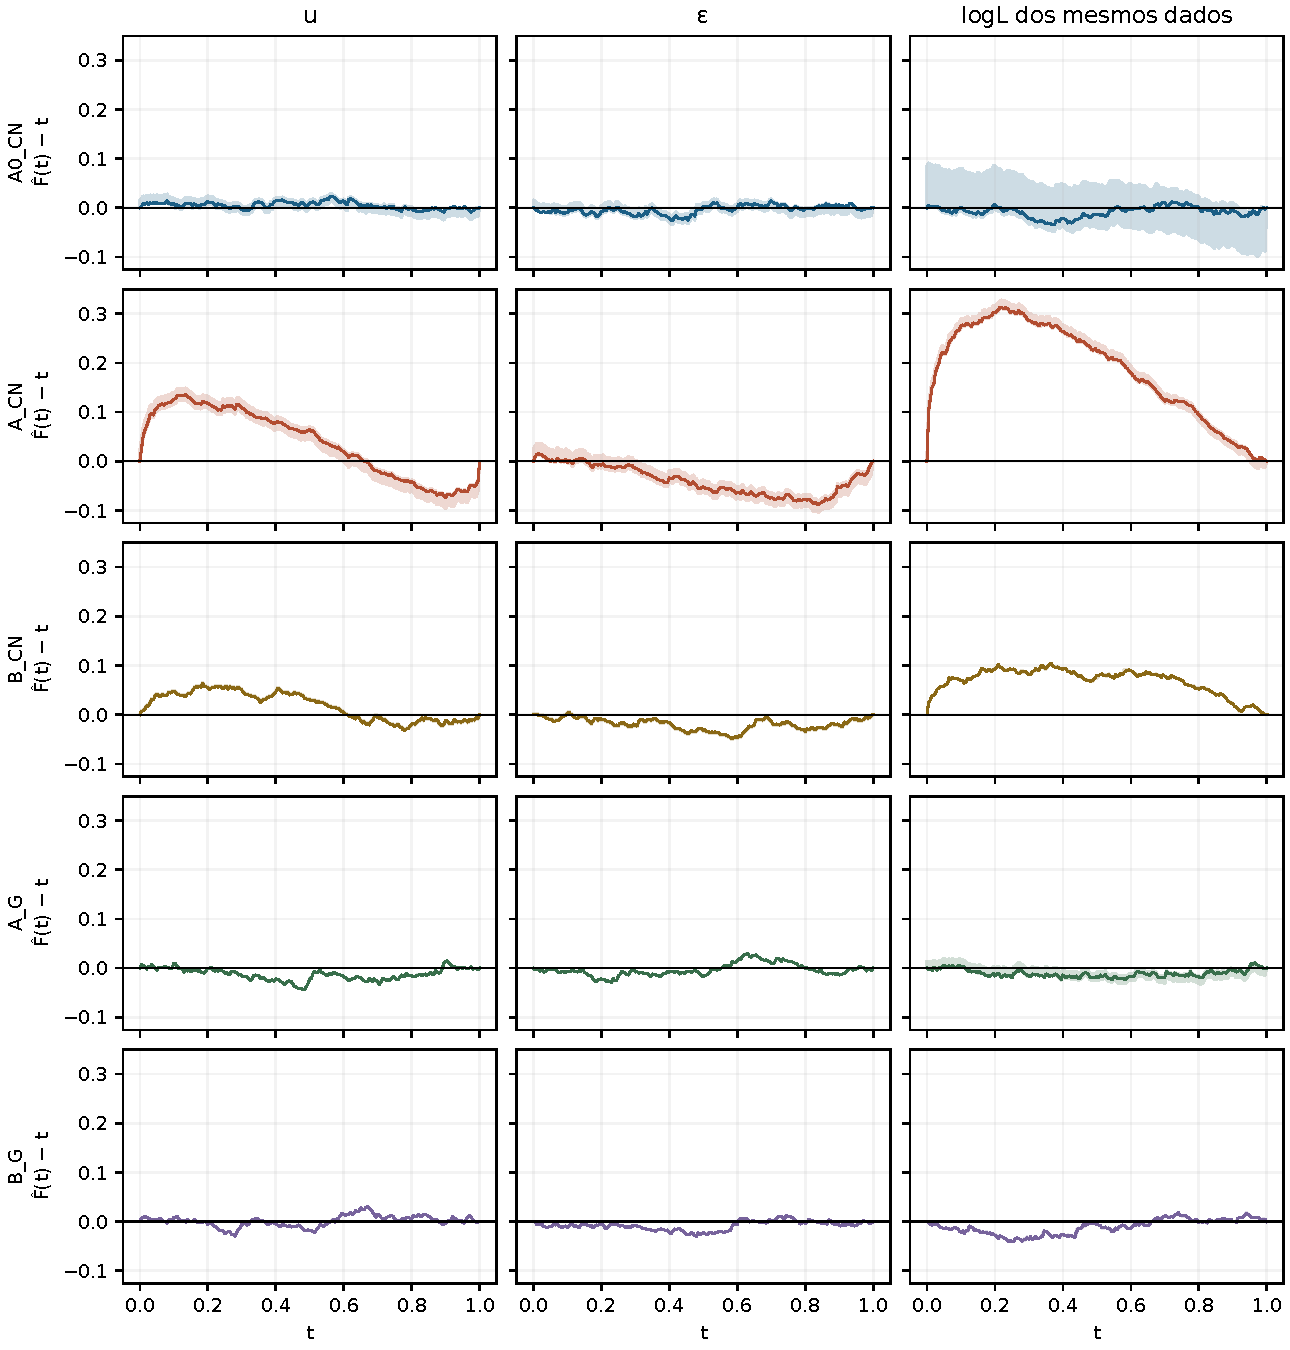
\includegraphics[width=\textwidth,height=.78\textheight,keepaspectratio]{../figures/escalar/sbc_ecdf.pdf}
\caption{Desvios das CDFs empíricas dos PITs em relação à uniforme.
Linhas: representação nominal; faixas: envelope das CDFs permitido pelos
intervalos numéricos, incluindo os casos $[0,1]$. Cada painel usa todos
os 500 dados da priori conjunta. A interpretação dos testes é dada pela
Tabela~\ref{tab:c10-sbc-familias}, com as correções de multiplicidade.}
\label{fig:c10-sbc}
\end{figure}

A cobertura central nominal de 90\% para $u$ foi 444/500 em A0\_CN,
365/500 em A\_CN e 422/500 em B\_CN. Os intervalos numéricos das contagens
foram, respectivamente, $[436,444]$, $[357,369]$ e $[421,422]$.
Nos controles A\_G e B\_G, as contagens foram 452/500 e 447/500,
sem ambiguidade nessa cobertura. Para $\varepsilon$, as contagens
nominais foram 454, 436, 451, 449 e 451, na mesma ordem de métodos.
A subcobertura de $u$ nas duas aproximações persistiu após Holm.
Isso evidencia uma limitação da normal aplicada aos estimadores físicos,
mesmo com seus primeiros dois momentos calculados corretamente.

Nas seis comparações pareadas de cobertura, houve quatro rejeições
nominais, das quais duas persistiram: A\_CN versus B\_CN e A0\_CN versus
A\_CN, ambas para $u$. As duas comparações correspondentes em
$\varepsilon$ ficaram indeterminadas. As comparações A\_G versus B\_G
não foram rejeitadas sob os intervalos. Esses testes avaliam cobertura;
não provam igualdade de informação ou de posteriores.

\subsection{Declarações sob a hipótese tensorial e recuperação}

Nas 500 injeções tensoriais, A0\_CN teve duas declarações nominais de
componente escalar, A\_CN teve 22 e B\_CN teve dez: taxas nominais de
0,4\%, 4,4\% e 2,0\%. A incerteza numérica amplia as contagens possíveis
para nove e 39 nos dois primeiros métodos. A Tabela~\ref{tab:c10-fp}
e a Figura~\ref{fig:c10-fp} conservam essa diferença entre contagem
nominal, decisão certa e decisão possível. As taxas descrevem o limiar
$\mathrm{BF}_{10}>10$ e a priori adotada; esse limiar não foi ajustado
para garantir uma taxa frequencista prefixada.

\begin{table}[htbp]
\centering
\caption{Declarações escalares nas injeções tensoriais. A última coluna
é a união dos intervalos exatos de Clopper--Pearson a 95\% sobre as
contagens numericamente possíveis, expressa em porcentagem.}
\label{tab:c10-fp}
\small\begin{tabular}{lrrrr}
\hline
Método & $N$ & Nominais & Certas/possíveis & IC 95\% (\%) \\
\hline
A0\_CN & 500 & 2 & [2, 9] & 0,05--3,39 \\
A\_CN & 500 & 22 & [22, 39] & 2,78--10,51 \\
B\_CN & 500 & 10 & [10, 10] & 0,96--3,65 \\
A\_G & 500 & 2 & [2, 3] & 0,05--1,74 \\
B\_G & 500 & 1 & [1, 1] & 0,01--1,11 \\
\hline
\end{tabular}

\end{table}

\begin{figure}[htbp]
\centering
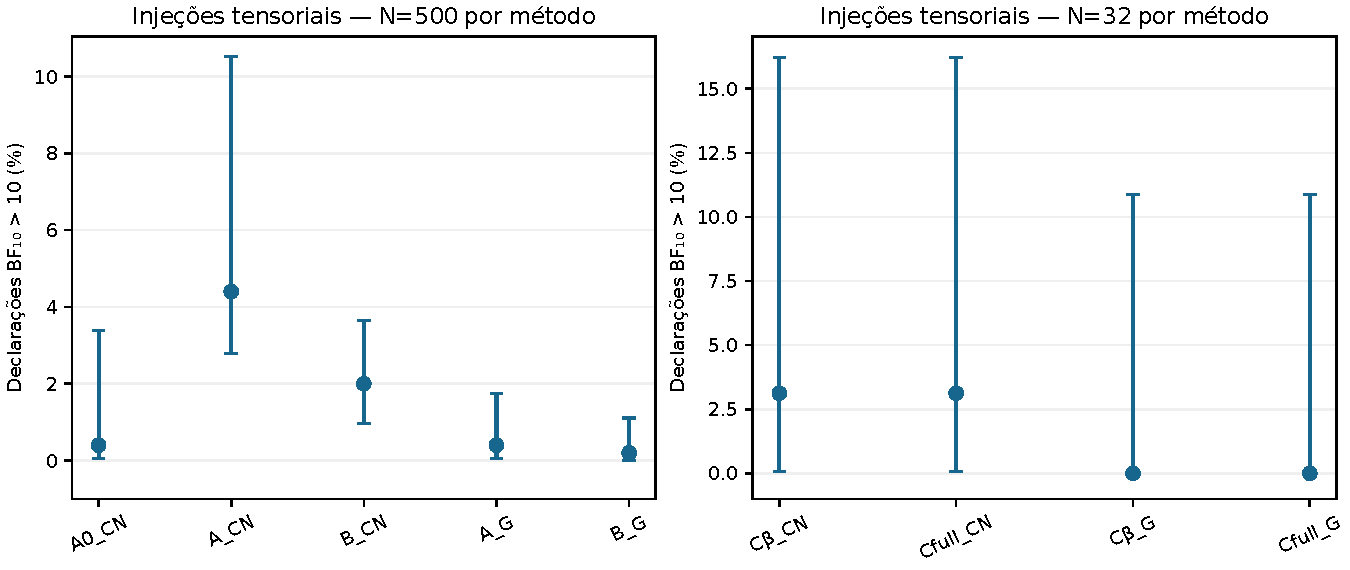
\includegraphics[width=\textwidth]{../figures/escalar/falsos_positivos.pdf}
\caption{Falsos positivos no limiar $\mathrm{BF}_{10}>10$.
Pontos: taxas nominais; barras: união dos intervalos binomiais a 95\%
considerando a sensibilidade numérica. Os painéis têm tamanhos amostrais
e escalas verticais diferentes. O subconjunto C tem finalidade descritiva.}
\label{fig:c10-fp}
\end{figure}

As células mistas apresentaram baixa frequência de declarações no domínio
examinado. Em $(u,\varepsilon)=(0{,}2,0{,}5)$, A0\_CN declarou três
casos em 32, com quatro possíveis; A\_G declarou oito e B\_G dois.
Nas duas células com $u=0{,}995$, todos os métodos D tiveram zero
declarações nominais, mas alguns intervalos permitiram declarações:
em A\_CN e $\varepsilon=0{,}1$, por exemplo, a contagem possível chegou
a oito. A Figura~\ref{fig:c10-recuperacao} conserva todas essas células.
As comparações de detecção são descritivas; não foi acrescentado um teste
pareado de poder após observar esses resultados.

\begin{figure}[htbp]
\centering
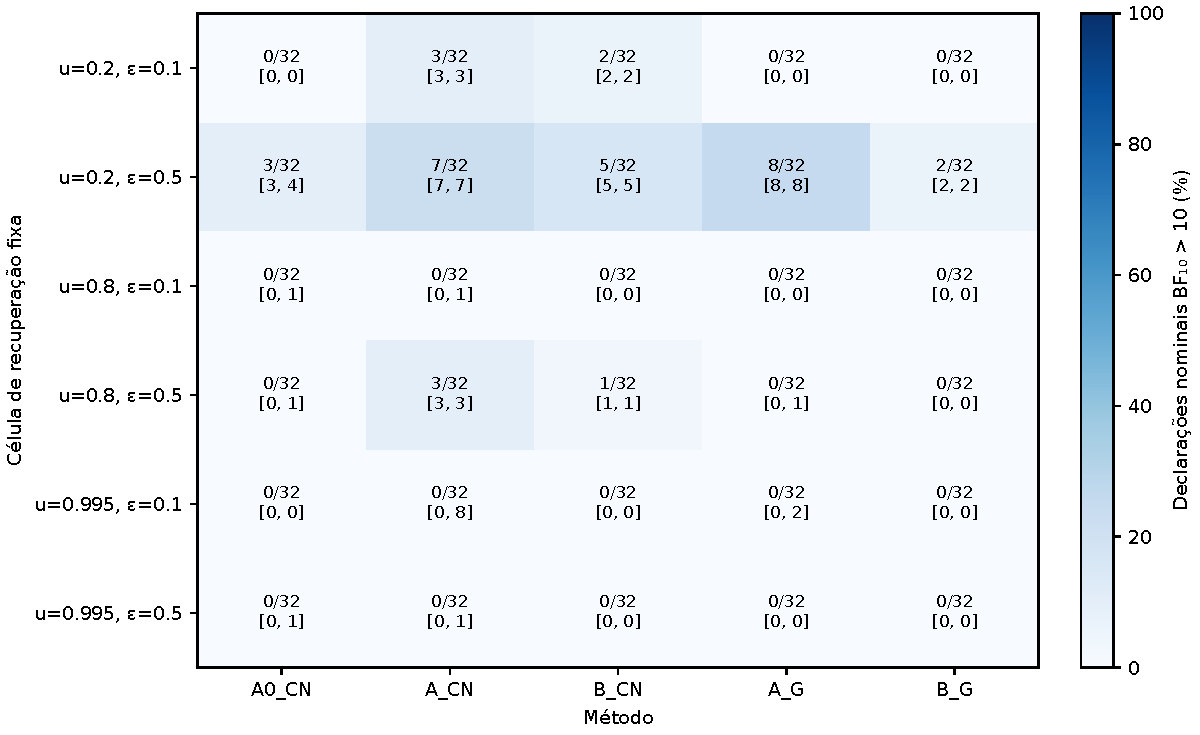
\includegraphics[width=\textwidth]{../figures/escalar/recuperacao_deteccao.pdf}
\caption{Declarações nas seis células de recuperação, com 32 realizações
por célula e método D. Cada entrada apresenta a contagem nominal sobre
32 e, entre colchetes, as contagens certa e possível. A cor representa
somente a frequência nominal. As células não são reunidas em um teste
binomial comum.}
\label{fig:c10-recuperacao}
\end{figure}

A recuperação dos parâmetros também é limitada perto da fronteira.
Em A0\_CN, para $u=0{,}995$ e $\varepsilon=0{,}1$ ou $0{,}5$,
as medianas das medianas posteriores de $u$ foram aproximadamente
0,795 e 0,716, e a cobertura central nominal foi 0/32 e 3/32.
São resultados condicionais em verdades fixas, não falhas automaticamente
rejeitáveis por um teste SBC de uniformidade. Eles mostram por que a
calibração média sobre a priori não garante boa recuperação em toda
célula, especialmente junto à fronteira do suporte.

O conjunto sustenta uma extensão metodológica delimitada: a resposta
escalar vinculada pode ser incorporada ao experimento, e a escolha da lei
aproximada altera a calibração, a cobertura e as declarações nominais.
Não sustenta a detecção de uma polarização adicional em dados reais,
uma nova restrição observacional de massa, nem a recuperação eficiente
em todo o domínio. As nuisances continuam fixas na campanha; suas
degenerescências são examinadas localmente a seguir.

\section{Degenerescências locais e perda de informação}

O diagnóstico físico de Fisher foi concluído nos oito pontos prospectivos, para A0\_CN, A\_G e B\_G. As seis coordenadas são
\begin{equation}
 \theta=(u,\varepsilon,\log_{10}A_T,\gamma,
 \log_{10}A_r,\log_{10}{\rm EFAC}).
\end{equation}
Para a CN própria, a informação é
\begin{equation}
 I_{ij}^{\rm CN}=\sum_n\operatorname{Re}\operatorname{tr}
 \bigl(C_n^{-1}C_{n,i}C_n^{-1}C_{n,j}\bigr).
\end{equation}
Para o experimento normal real, acrescenta-se o termo de média e aparece o fator $1/2$ no termo de covariância:
\begin{equation}
 I_{ij}^{\rm G}=\sum_n\left[
 \mu_{n,i}^{T}\Sigma_n^{-1}\mu_{n,j}
 +\frac12\operatorname{tr}
 (\Sigma_n^{-1}\Sigma_{n,i}\Sigma_n^{-1}\Sigma_{n,j})\right].
\end{equation}
Em B\_G, a soma de canais é substituída pela média e covariância do vetor comprimido com os pesos fixos. Não se atribui essa Fisher normal à distribuição física exata dos estimadores quadráticos.

As diferenças finitas foram refinadas até o passo relativo $1{,}953125\times10^{-6}$, com estênceis unilaterais nas fronteiras. Perto de $u=0{,}995$ e de $u=1$, os passos iniciais não eram suficientes. A antissimetria de arredondamento foi medida e removida antes da aplicação da identidade hermitiana; a projeção das derivadas foi limitada pela escala do erro da diferença finita, sem modificar autovalores para reparar positividade. As tentativas rejeitadas pelos controles estão preservadas no histórico computacional.

As 24 matrizes passaram nos critérios de mudança relativa inferior a $10^{-3}$, refinamento harmônico e estabilidade do posto entre os dois últimos passos. Uma reconstrução independente por traços e pela regra da cadeia apresentou diferença relativa máxima de $1{,}89\times10^{-5}$. A informação das quatro nuisances foi projetada pelo espaço dos escores, conservando direções singulares sem inversão artificial.

Nas seis células de recuperação, os três métodos tiveram posto numérico seis nas escalas declaradas. Em $u=0{,}001$, B\_G apresentou posto cinco; em $u=1$, A0\_CN apresentou posto quatro. Esses postos usam limiar relativo $10^{-8}$ e não constituem prova de não identificabilidade exata. O forte condicionamento nas fronteiras exige distinguir um diagnóstico numérico local de uma afirmação física global.

\begin{figure}[htbp]
 \centering
 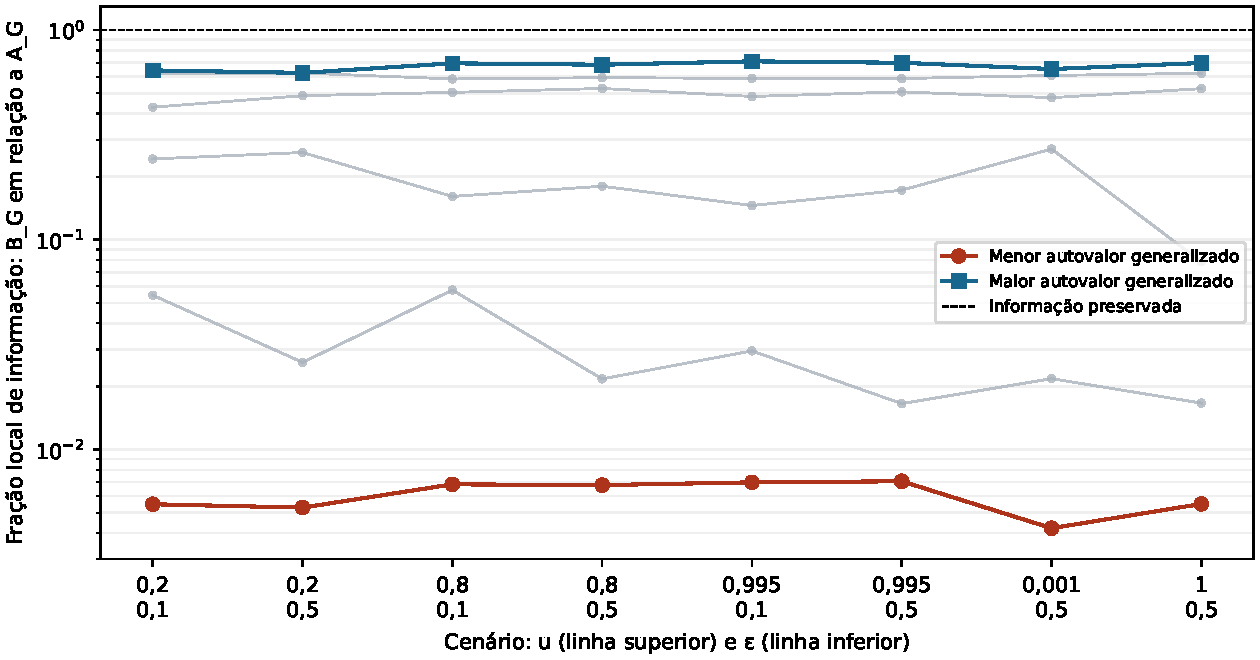
\includegraphics[width=\textwidth]{../figures/escalar/fisher_compressao.pdf}
 \caption{Autovalores generalizados de $I_{B\_G}v=\lambda I_{A\_G}v$ nos oito cenários. As curvas cinzas mostram os quatro autovalores intermediários. A comparação é entre o experimento normal por frequência e sua compressão linear, com seis coordenadas e geometria fixas; não é uma comparação de evidências ou de A0\_CN com uma lei aproximada.}
 \label{fig:fisher-escalar-compressao}
\end{figure}

A Figura~\ref{fig:fisher-escalar-compressao} quantifica a perda local de informação pela compressão dentro do experimento G. Os menores autovalores ficam entre 0,0042 e 0,0071; os maiores, entre 0,625 e 0,710. Assim, há combinações locais dos seis parâmetros que conservam menos de 1\% da informação, embora outras direções conservem uma fração maior. Isso não significa que um parâmetro isolado, como $u$, perca necessariamente a mesma fração. Os resultados dependem deste experimento e não substituem a recuperação populacional nem uma posterior com nuisances livres. C10 conclui a extensão condicional prevista, conservando as indeterminações numéricas e as limitações de recuperação descritas neste capítulo.
